\subsection{Ethereum}
\label{subsec:ethereum}

Ethereum adalah sebuah platform berbasis Blockchain untuk membangun aplikasi terdesentralisasi dan Smart Contracts, dengan serangkaian \textit{tradeoffs} yang berbeda. Dikembangkan oleh Vitalik Buterin pada tahun 2015, Ethereum mengembangkan konsep dasar Blockchain dengan menambahkan sebuah bahasa pemrograman \textit{Turing-complete} untuk mengembangkan Smart Contracts, yang dijalankan di dalam Ethereum Virtual Machine (EVM). Ethereum Virtual Machine (EVM) adalah sebuah lingkungan eksekusi untuk Smart Contracts di Ethereum, yang memungkinkan kode berjalan di seluruh jaringan Ethereum secara terdistribusi. Bahasa pemrograman bawaan Ethereum yang \textit{Turing-complete} adalah Solidity, yang digunakan untuk menulis Smart Contracts di Ethereum. Solidity adalah bahasa dengan paradigma berorientasi objek, seluruh program Smart Contract akan dikompilasi menjadi sebuah \textit{byte-code}, dalam kasus ini menjadi bentuk EVM Bytecode, dan spesifikasinya dituliskan pada sebuah Application Binary Interface (ABI). Dengan bahasa pemrograman yang \textit{Turing-complete} dan mekanisme eksekusi yang terjamin dengan EVM, Ethereum memberikan kemampuan bagi pengembang untuk mengembangkan sebuah aplikasi yang terdesentralisasi, yang disebut juga sebagai \textit{dApps}, di mana kode dan data disimpan di dalam Blockchain, sehingga mendapatkan karakteristik bawaan dari karakteristik Blockchain \parencite{buterin2013ethereum}.

\subsubsection{ABI}
\label{subsubsec:abi}

\begin{figure}[ht]
  \centering
  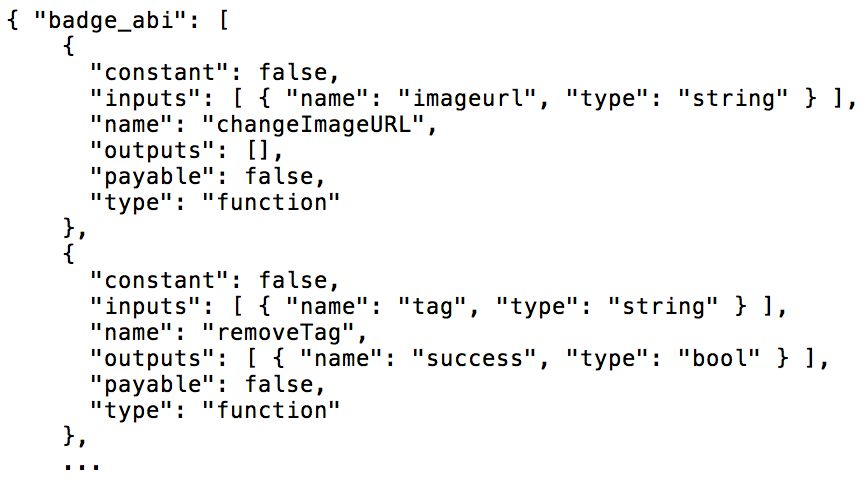
\includegraphics[width=0.7\textwidth]{resources/chapter-2/smart-contract-abi.jpg}
  \caption{Contoh ABI dari sebuah Smart Contract \parencite{third2017linked}}
  \label{image:abi-example}
\end{figure}

Application Binary Interface (ABI) adalah sebuah konvensi yang mendefinisikan aspek-aspek kode yang dihasilkan selama kompilasi, seperti representasi data, penggunaan register, dan konvensi pemanggilan fungsi \parencite{sciencedirect2024}. Dalam konteks Smart Contracts yang ditulis dengan bahasa Solidity dan dikompilasi, hasil dari kompilasinya akan berbentuk EVM Bytecode untuk dieksekusi di dalam EVM, disertai dengan ABI yang mendefinisikan Smart Contract tersebut, seperti pada gambar \ref{image:abi-example}.

\subsubsection{Decentralized Applications (dApps)}
\label{subsubsec:dapps}

Decentralized Applications (dApps) adalah sebuah aplikasi yang berjalan di atas infrastruktur Blockchain dengan memanfaatkan Smart Contracts untuk menyediakan fungsionalitasnya. Karena dApps berjalan di atas Blockchain, dApps mewarisi sifat-sifat yang inheren dari Blockchain, seperti terdesentralisasi, \textit{immutable}, transparan, dan sifat-sifat lainnya \parencite{investopedia2024}. dApps tidak berbeda dari aplikasi tradisional dari sisi pengguna, perbedaannya hanya terletak pada komputasi dari fungsionalitas yang diberikan oleh dApps dilakukan menggunakan Smart Contracts dan seluruh datanya terletak di dalam Blockchain \parencite{metcalfe2020ethereum}. 

\subsubsection{Etherscan}
\label{subsubsec:etherscan}

Etherscan adalah sebuah \textit{block explorer}, \textit{search engine} untuk pengguna agar dapat dengan mudah melihat, mengonfirmasi, dan memvalidasi transaksi untuk Blockchain Ethereum. Etherscan didirikan oleh Matthew Tan pada tahun 2015, dan berdiri secara independen dari Ethereum Foundation. Etherscan melakukan \textit{indexing} terhadap Blockchain untuk menampilkan informasinya, di mana informasi tersebut digunakan untuk menyediakan API untuk pengembang mengintegrasikan informasi Blockchain Ethereum ke dalam aplikasinya \parencite{etherscan2024}.